\documentclass[12pt]{beamer}
\newenvironment{ConCodigo}[1]
  {\begin{frame}[fragile,environment=ConCodigo]{#1}}
  {\end{frame}}
\graphicspath{{Imagenes/}{../Imagenes/}}
\usepackage[utf8]{inputenc}
\usepackage[spanish]{babel}
\usepackage{hyperref}
\usepackage{etex}
%\reserveinserts{28}
\usepackage{amsmath}
\usepackage{amsthm}
\usepackage{mathtools}
\usepackage{multicol}
\usepackage{multirow}
\usepackage{tabulary}
\usepackage{booktabs}
\usepackage{nccmath}
\usepackage{physics}
\usepackage{biblatex}
\usepackage[outdir=./]{epstopdf}
%\epstopdfsetup{outdir=./}
\usepackage{graphicx}
%\usepackage{enumitem,xcolor}
\usepackage{siunitx}
%\sisetup{scientific-notation=true}
%\usepackage{fontspec}
\usepackage{lmodern}
\usepackage{float}
\usepackage[format=hang, font=footnotesize, labelformat=parens]{caption}
\usepackage[autostyle,spanish=mexican]{csquotes}
\usepackage{standalone}
\usepackage{blkarray}
\usepackage{algorithm}
\usepackage{algorithmic}
\usepackage{tikz}
\usepackage[siunitx, RPvoltages]{circuitikz}
\usetikzlibrary{arrows,patterns,shapes}
\usetikzlibrary{decorations.markings}
\usetikzlibrary{arrows}
\usepackage{color}
\usepackage{xcolor}
%\usepackage{beton}
%\usepackage{euler}
%\usepackage[T1]{fontenc}
\usepackage[sfdefault]{roboto}  %% Option 'sfdefault' only if the base font of the document is to be sans serif
\usepackage[T1]{fontenc}
\renewcommand*\familydefault{\sfdefault}
\DeclareGraphicsExtensions{.pdf,.png,.jpg}
\usepackage{hyperref}
\renewcommand {\arraystretch}{1.5}
\newcommand{\python}{\texttt{python}}
\usefonttheme[onlymath]{serif}
\setbeamertemplate{navigation symbols}{}
\usetikzlibrary{patterns}
\usetikzlibrary{decorations.markings}
\tikzstyle{every picture}+=[remember picture,baseline]
%\tikzstyle{every node}+=[inner sep=0pt,anchor=base,
%minimum width=2.2cm,align=center,text depth=.15ex,outer sep=1.5pt]
%\tikzstyle{every path}+=[thick, rounded corners]
\setbeamertemplate{caption}[numbered]
\newcommand{\ptm}{\fontfamily{ptm}\selectfont}
%Se usa la plantilla Warsaw modificada con spruce
\mode<presentation>
{
  \usetheme{Warsaw}
  \setbeamertemplate{headline}{}
  \useoutertheme{default}
  \usecolortheme{albatross}
  \setbeamercovered{invisible}
}
% \AtBeginSection[]
% {
% \begin{frame}<beamer>{Contenido}
% \normalfont\mdseries
% \tableofcontents[currentsection]
% \end{frame}
% }

\input{../Preambulos/pre_codigo}
%Se usa la plantilla Warsaw modificada con spruce
\mode<presentation>
{
  \usetheme{Warsaw}
  \setbeamertemplate{headline}{}
  \useoutertheme{default}
  \usecolortheme{seahorse}
  \setbeamercovered{invisible}

  \setbeamertemplate{section in toc}[sections numb
  \setbeamertemplate{subsection in toc}[subsection
  \setbeamertemplate{subsection in toc}{\leavevmode\leftskip=3.2em\rlap{\hskip-2em\inserttocsectionnumber.
  \inserttocsubsectionnumber}\inserttocsubsection\
  \setbeamercolor{section in toc}{fg=blue}
  \setbeamercolor{subsection in toc}{fg=blue}
  \setbeamerfont{subsection in toc}{size=\small}

}
% \AtBeginSection[]
% {
% \begin{frame}<beamer>{Contenido}
% \normalfont\mdseries
% \tableofcontents[currentsection]
% \end{frame}
%}
\makeatletter
\setbeamertemplate{footline}
%\setbeamercolor{title in head/foot}{fg=Green}
{
  \leavevmode%
  \hbox{%
  \begin{beamercolorbox}[wd=.333333\paperwidth,ht=2.25ex,dp=1ex,center]{author in head/foot}%
    \usebeamerfont{author in head/foot} \textcolor{white}{\insertsection}
  \end{beamercolorbox}}%
  \begin{beamercolorbox}[wd=.333333\paperwidth,ht=2.25ex,dp=1ex,center]{title in head/foot}%
    \usebeamerfont{title in head/foot} \textcolor{white}\insertsubsection
  \end{beamercolorbox}%
  \begin{beamercolorbox}[wd=.333333\paperwidth,ht=2.25ex,dp=1ex,right]{date in head/foot}%
    \usebeamerfont{date in head/foot} \textcolor{white}\insertshortdate{}\hspace*{2em}
    \textcolor{white}\insertframenumber{} / \textcolor{white}\inserttotalframenumber\hspace*{2ex} 
  \end{beamercolorbox}}%
  \vskip0pt%
\makeatother
\normalfont
\usepackage{ccfonts}% http://ctan.org/pkg/{ccfonts}
\usepackage[T1]{fontenc}% http://ctan.or/pkg/fontenc
\renewcommand{\rmdefault}{cmr}% cmr = Computer Modern Roman
\linespread{1.3}
\title{Métodos de Monte Carlo}
\subtitle{Curso de Física Computacional}
\author[]{M. en C. Gustavo Contreras Mayén}
% \newcounter{saveenumi}
% \newcommand{\seti}{\setcounter{saveenumi}{\value{enumi}}}
% \newcommand{\conti}{\setcounter{enumi}{\value{saveenumi}}}
% \resetcounteronoverlays{saveenumi}
\setbeamercolor*{block body}{fg=white,bg=black!10}
\author{M. en C. Gustavo Contreras Mayén}
\date{\today}
\institute{Facultad de Ciencias - UNAM}
\titlegraphic{\includegraphics[width=1.75cm]{escudo-facultad-ciencias.jpg}\hspace*{4.75cm}~%
   \includegraphics[width=1.75cm]{escudo-unam.jpg}
}
\begin{document}
\maketitle
\fontsize{14}{14}\selectfont
\spanishdecimal{.}
\newcommand{\localtextbulletone}{\textcolor{gray}{\raisebox{.45ex}{\rule{.6ex}{.6ex}}}}
\section*{Contenido}
\frame{\tableofcontents[currentsection, hideallsubsections]}
\section{Métodos de Monte Carlo}
\frame{\tableofcontents[currentsection, hideothersubsections]}
\subsection{Definición}
\begin{frame}
\frametitle{Definición}
El método Monte Carlo es un conjunto de métodos numéricos que permiten resolver problemas físicos y matemáticos mediante la simulación de variables aleatorias.
\end{frame}
\begin{frame}
\frametitle{Definición}
Los métodos Monte Carlo fueron nombrados de esta manera por su clara analogía con los juegos de ruleta de los casinos, el más célebre de los cuales es el de Montecarlo, casino cuya construcción fue propuesta en 1856 por el príncipe Carlos III de Mónaco, siendo inaugurado en 1861.
\end{frame}
\begin{frame}
\frametitle{Relevancia del método}
La importancia actual de los métodos Monte Carlo se basa en la existencia de problemas que tienen difícil solución por métodos exclusivamente analíticos o numéricos, pero que dependen de factores aleatorios o se pueden asociar a un modelo probabilístico artificial (resolución de integrales de muchas variables, minimización de funciones, etc.)
\end{frame}
\begin{frame}
\frametitle{Relevancia del método}
Gracias al continuo diseño de procesadores y de computadoras, los cálculos con Monte Carlo que en otro tiempo hubieran sido inconcebibles, hoy en día se presentan como asequibles para la resolución de ciertos problemas.
\end{frame}
\begin{frame}
 \frametitle{Proporción del error}
En estos métodos el error $\simeq \frac{1}{\sqrt{N}}$, donde $N$ es el número de pruebas, por tanto, ganar una cifra decimal en la precisión implica aumentar $N$ en $100$ veces.
\end{frame}
\begin{frame}
 \frametitle{Fundamento del método}
La base del método es la generación de números aleatorios de los que nos serviremos para calcular probabilidades.
\\
\bigskip
Conseguir un buen generador de estos números así como un conjunto estadístico adecuado sobre el que trabajar son las primeras dificultades con la nos vamos a encontrar a la hora de utilizar este método.
\end{frame}
\subsection{Secuencia aleatoria}
\begin{frame}
\frametitle{Secuencia aleatoria}
Se define una secuencia aleatoria de números $r_{1}, r_{2}, \ldots$ si no existe una correlación entre ellos.
\\
\bigskip
Aunque sean aleatorios, no implica que todos los números en la secuencia tengan la misma probabilidad de ocurrir.
\end{frame}
\begin{frame}
\frametitle{Secuencia aleatoria}
Si todos los números en la secuencia tienen la misma probabilidad de ocurrir, se dice que la secuencia es \textcolor{blue}{uniforme} y los \textcolor{red}{números son aleatorios}.
\\
\bigskip
Por ejemplo: $1, 2, 3, 4, \ldots$ es uniforme pero probablemente no es aleatoria.
\end{frame}
\begin{frame}
\frametitle{Secuencia aleatoria}
También es posible tener una secuencia de números que de alguna forma son aleatorios, pero tienen correlación dentro de un intervalo pequeño:
\[ r_{1},  \: (1 - r_{1} ), \: r_{2}, \: (1 - r_{2} ), \: r_{3}, \: (1 - r_{3} ), \: \ldots  \]
Las computadoras por naturaleza, son determinísticas y no pueden crear una secuencia de números aleatorios.
\end{frame}
\begin{frame}
\frametitle{Secuencia aleatoria}
Las computadoras pueden crear secuencias que contengan correlaciones y por tanto no ser totalmente aleatorias; si conocemos $r_{m}$ y su elemento precedente, es posible estimar $r_{m+1}$.
\\
\bigskip
Por ésta razón, se dice que las computadoras son generadores de números pseudo-aleatorios.
\end{frame}
\begin{frame}
\frametitle{Secuencia aleatoria}
Matemáticamente, la probabilidad de que un número ocurra, está descrita por una función de distribución $P(r)$, donde $P(r) \: dr$, es la probabilidad de encontrar $r$ en un intervalo $[r, r + dr]$.
\\
\bigskip
Una distribución uniforme significa que $P(r) = \mbox{ constante}$.
\end{frame}
\begin{frame}
\frametitle{Generador de número aleatorios}
El generador estándar de números aleatorios en las computadoras, genera distribuciones uniformes entre $0$ y $1$.
\\
\bigskip
El generador estándar de números aleatorios, proporciona números en éste intervalo, y cada uno de ellos tiene la misma probabilidad de ocurrir, y además es independiente del número anterior.
\end{frame}
\subsection{Generación de números aleatorios}
\begin{frame}
\frametitle{Generación de números aleatorios}
El método de \emph{congruencia lineal} es la manera más común que se utiliza para generar una
secuencia de números pseudo-aleatorios $0 \leq r_{i} \leq M - 1$ en el intervalo $[0, M -1]$.
\end{frame}
\begin{frame}
\frametitle{Generación de números aleatorios}
Podemos multiplicar el número aleatorio previo $r_{i-1}$ por una constante $a$, sumar otra constante $c$, operar con el módulo $M$, manteniendo sólo la parte fraccional del resultado como el siguiente número aleatorio $r_{i+1}$
\[ r_{i+1} = (a \; r_{i} + c) \mbox{ mod } M \]
\end{frame}
\begin{frame}
\[ r_{i+1} = (a \; r_{i} + c) \mbox{ mod } M \]
El valor de $r_{1}$ se le llama \emph{semilla} (\textcolor{blue}{seed}, en inglés) y lo proporciona normalmente el usuario.
\end{frame}
\begin{frame}
\frametitle{Ejemplo}
Veamos la secuencia que se genera si $c = 1$, $a = 4$, $M = 9$, y la semilla es $r_{1} = 3$:
\[ r_{i+1} = (a \; r_{i} + c) \mbox{ mod } M \]
\begin{align*}
r_{1} &= 3 \\
r_{2} &= (4 \times 3  + 1) \mbox{ mod } 9 = 13 \mbox{ mod } 9 = 4 \\
r_{3} &= (4 \times 4  + 1) \mbox{ mod } 9 = 17 \mbox{ mod } 9 = 8 \\
r_{4} &= (4 \times 8  + 1) \mbox{ mod } 9 = 33 \mbox{ mod } 9 = 6 \\
r_{5 - 10} &= 7, 2, 0, 1, 5, 3
\end{align*}
\end{frame}
\begin{frame}
Hemos obtenido una secuencia de longitud $M = 9$, antes de que la secuencia se repitiera.
\\
\bigskip
Si queremos números en el rango $[0, 1]$, basta dividir los números $r$ por $M = 9$:
\[ \begin{split}
0.333, 0.222, 0.444, 0.000, 0.889, \\
0.111, 0.667, 0.555, 0.778, 0.333 \end{split} \]
\end{frame}
\begin{frame}
Aún sigue siendo una secuencia de longitud $9$ pero ya no es una secuencia de enteros.
\\
\bigskip
Si queremos que los números aleatorios estén en el rango $[A, B]$, se requiere aplicar el factor de escala:
\[ x_{i} = A + (B - A) \; r_{i} \hspace{1cm} 0 \leq r_{1} \leq 1 \rightarrow A \leq x_{i} \leq B \]
\end{frame}
\begin{frame}
\frametitle{Sugerencia}
Antes de utilizar un generador de números aleatorios en nuestros programas, debemos de revisar que el rango que produce, tiene apariencia de aleatorios.
\end{frame}
\begin{frame}
\frametitle{Sugerencia}
Propiamente no es un prueba matemática, pero al graficar la distribución de números aleatorios, podemos reconocer ciertos patrones, con lo que nos diría si tenemos o no, números aleatorios.
\end{frame}
\begin{frame}[plain, allowframebreaks, fragile]
\frametitle{Código para los números aleatorios}
\begin{lstlisting}[caption=Código distribución, style=FormattedNumber, basicstyle=\linespread{1.1}\ttfamily=\small, columns=fullflexible]
x = []

a, semilla, c, m, n = 128, 10, 0, 509, 500
for i in range (1, n):
   nuevasemilla = (a * semilla + c) % m
   semilla = nuevasemilla
   x.append( nuevasemilla)

y = []

a, semilla, c, m, n = 269, 10, 0, 2048, 500

for i in range (1, n):
   nuevasemilla = (a * semilla + c) % m
   semilla = nuevasemilla
   y.append( nuevasemilla)
\end{lstlisting}
\end{frame}
\begin{frame}[fragile]
\frametitle{Distribución de números aleatorios (1/2)}
\begin{figure}
  \centering
  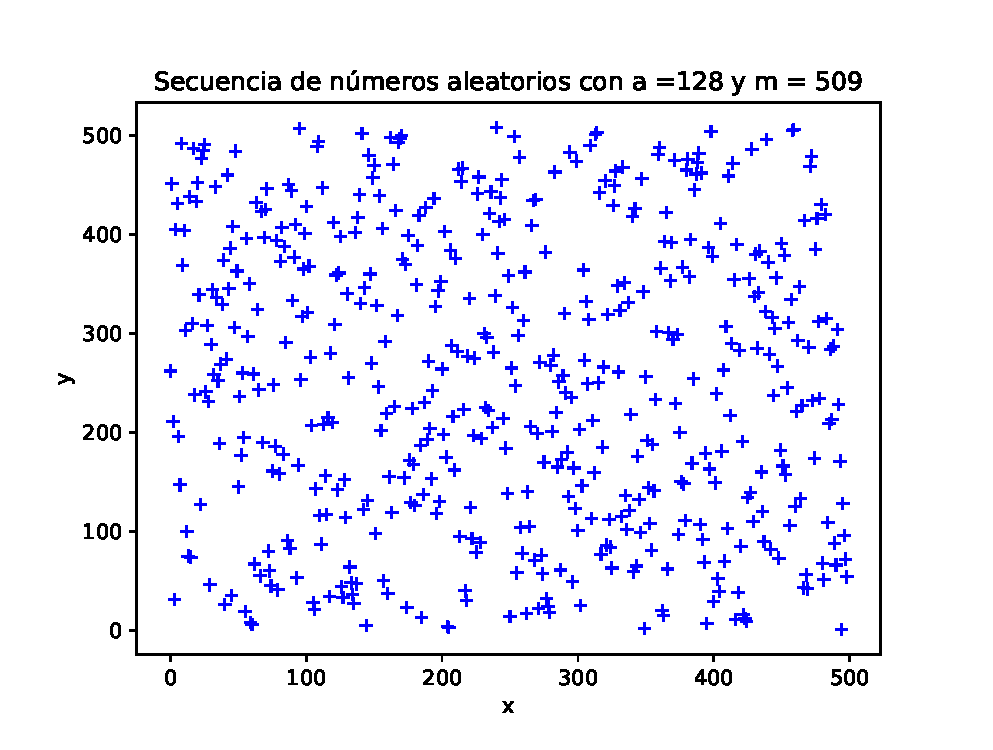
\includegraphics[scale=0.6]{Secuencia_aleatoria_01.eps}
\end{figure}
\end{frame}
\begin{frame}[fragile]
\frametitle{Distribución de números aleatorios (1/2)}
\begin{figure}
  \centering
  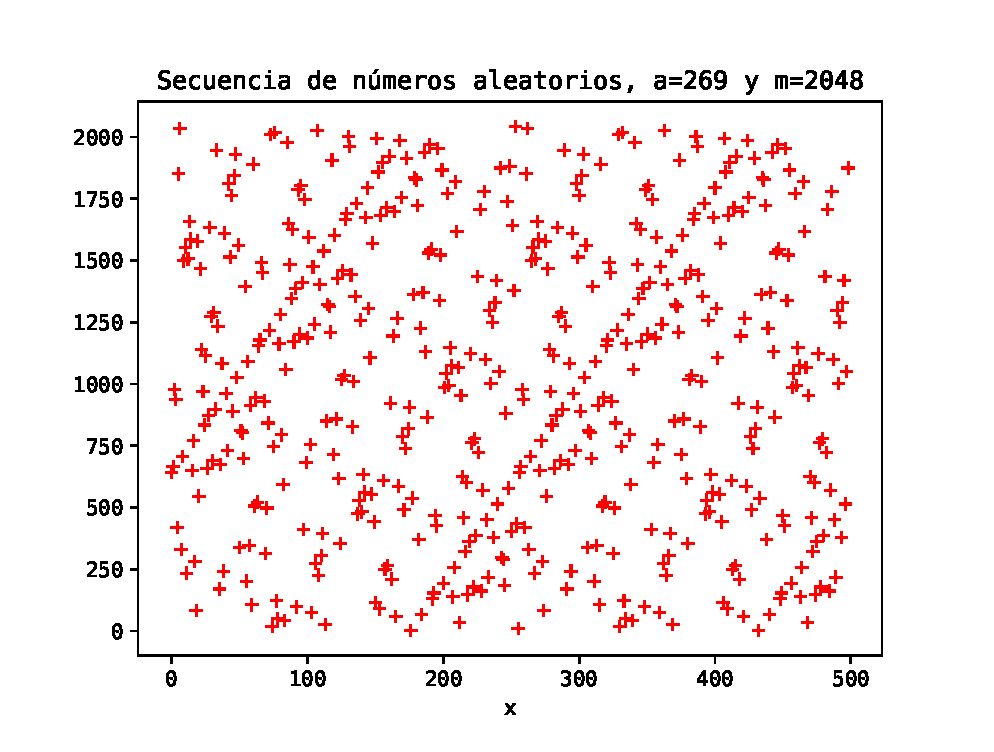
\includegraphics[scale=0.6]{Secuencia_aleatoria_02.eps}
\end{figure}
\end{frame}
\begin{frame}
\frametitle{La librería \texttt{random}}
Este módulo implementa generadores de números pseudoaleatorios para diversas distribuciones.
\\
\bigskip
Para números enteros, hay selección uniforme de un rango. Para las secuencias, hay una selección uniforme de un elemento aleatorio, una función para generar una permutación aleatoria de una lista \emph{in situ} y una función para el muestreo aleatorio sin reemplazo.
\end{frame}
\begin{frame}
\frametitle{La librería \texttt{random}}
Casi todas las funciones de la librería dependen de la función básica \funcionazul{random ()}, que genera un número flotante aleatorio de manera uniforme en el rango semiabierto $[0.0, 1.0)$
\end{frame}
\begin{frame}
\frametitle{La librería \texttt{random}}
En \python{} se usa el algoritmo \textoazul{Mersenne Twister} como generador central. Produce números flotantes de precisión de $53$ bits y tiene un período de $2^{19937}-1$.
\end{frame}
\begin{frame}
\frametitle{Alcance del generador en \texttt{random}}
El algoritmo \textoazul{Mersenne Twister} es uno de los generadores de números aleatorios más probados que existen.
\\
\bigskip
Sin embargo, al ser completamente determinista, no es adecuado para todos los propósitos, y es completamente inadecuado para fines criptográficos.
\end{frame}
\begin{frame}
\frametitle{Funciones importantes}
Dentro de la librería \funcionazul{random} existen distintas funciones que podremos utilizar, basta con revisar la documentación disponible, para identificar los parámetros y la respuesta que devuelve.
\end{frame}
\begin{frame}
\frametitle{Funciones importantes}
Mencionaremos dos funciones:
\setbeamercolor{item projected}{bg=green!70!black,fg=white}
\setbeamertemplate{enumerate items}[circle]
\begin{enumerate}[<+->]
\item \funcionazul{random.seed(a=None)}. Inicializa el generador de números aleatorios. Si no se especifica el valor de $a$, se utiliza el reloj del sistema. En caso de que $a$ sea un entero, se utilza directamente.
\item \funcionazul{random.random()}. Devuelve un número de punto flotante en el rango $[0.0, 1.0)$.
\end{enumerate}
\end{frame}
\begin{frame}
\frametitle{Ejemplo con \texttt{random.seed(a)}}
Haremos un ejercicio en donde se van a generar tres secuencias de números con la función \funcionazul{random.seed(a)}, cambiaremos el valor de la semilla y vamos a comparar los resultados en una gráfica.
\end{frame}
\begin{frame}[plain, allowframebreaks, fragile]
\frametitle{Código usando \texttt{seed()}}
\begin{lstlisting}[caption=Código con semilla, style=FormattedNumber, basicstyle=\linespread{1.1}\ttfamily=\small, columns=fullflexible]
import matplotlib.pyplot as plt
import random

def arreglonumeros(muestra=500, semilla=None):
    x = []
    random.seed(semilla)
    
    for i in range(muestra):
        nuevoValor = random.random()
        x.append(nuevoValor)
    
    return x

x_1_ = arreglonumeros()
x_2_ = arreglonumeros(semilla=500)
x_3_ = arreglonumeros(semilla=2018)

plt.figure(figsize=(8,5)) 
plt.plot(x_1_,'b+', label='seed = reloj sistema')
plt.plot(x_2_,'r+', label='seed = 500')
plt.plot(x_3_,'y+', label='seed = 2018')
plt.legend(loc='upper center', bbox_\textunderscore_to_\textunderscore_anchor=(0.93, 1.1), borderaxespad = 0.)
plt.title('Secuencia de numeros aleatorios')
plt.xlabel('x')
plt.ylabel('y')
plt.show()
\end{lstlisting}
\end{frame}
\begin{frame}[fragile]
\frametitle{Gráfica obtenida}
\begin{figure}
  \centering
  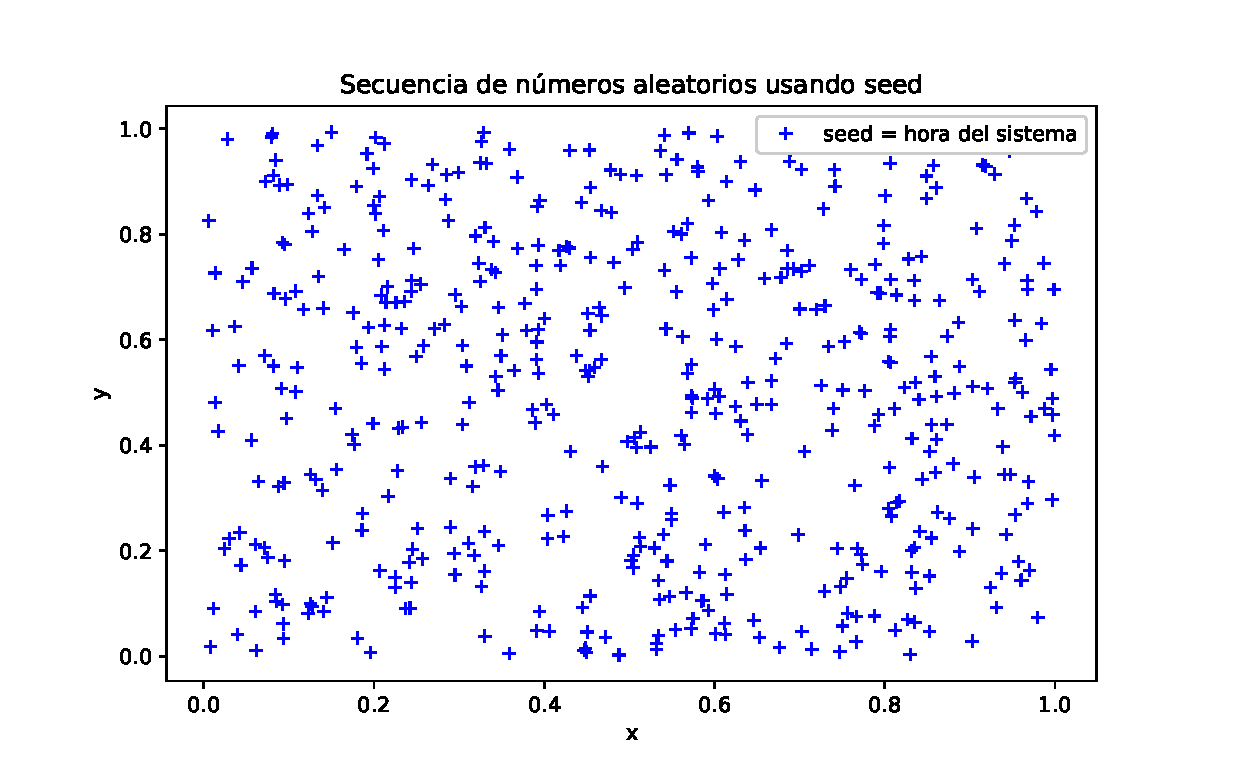
\includegraphics[scale=0.55]{Secuencia_aleatoria_04.eps}
\end{figure}
\end{frame}
\section{La aguja de Buffon}
\frame{\tableofcontents[currentsection, hideothersubsections]}
\subsection{Planteamiento}
\begin{frame}
\frametitle{La aguja de Buffon}
Resulta que $\pi$ también desempeña un papel importante en un experimento llamado \enquote{el problema de la aguja de Buffon}.
\\
\bigskip
El cual buscar determinar la probabilidad de que una aguja de longitud $\ell$, arrojada aleatoriamente aterrice en medio o atravesando una serie de líneas paralelas en el suelo.
\end{frame}
\begin{frame}
\begin{figure}
	\centering
	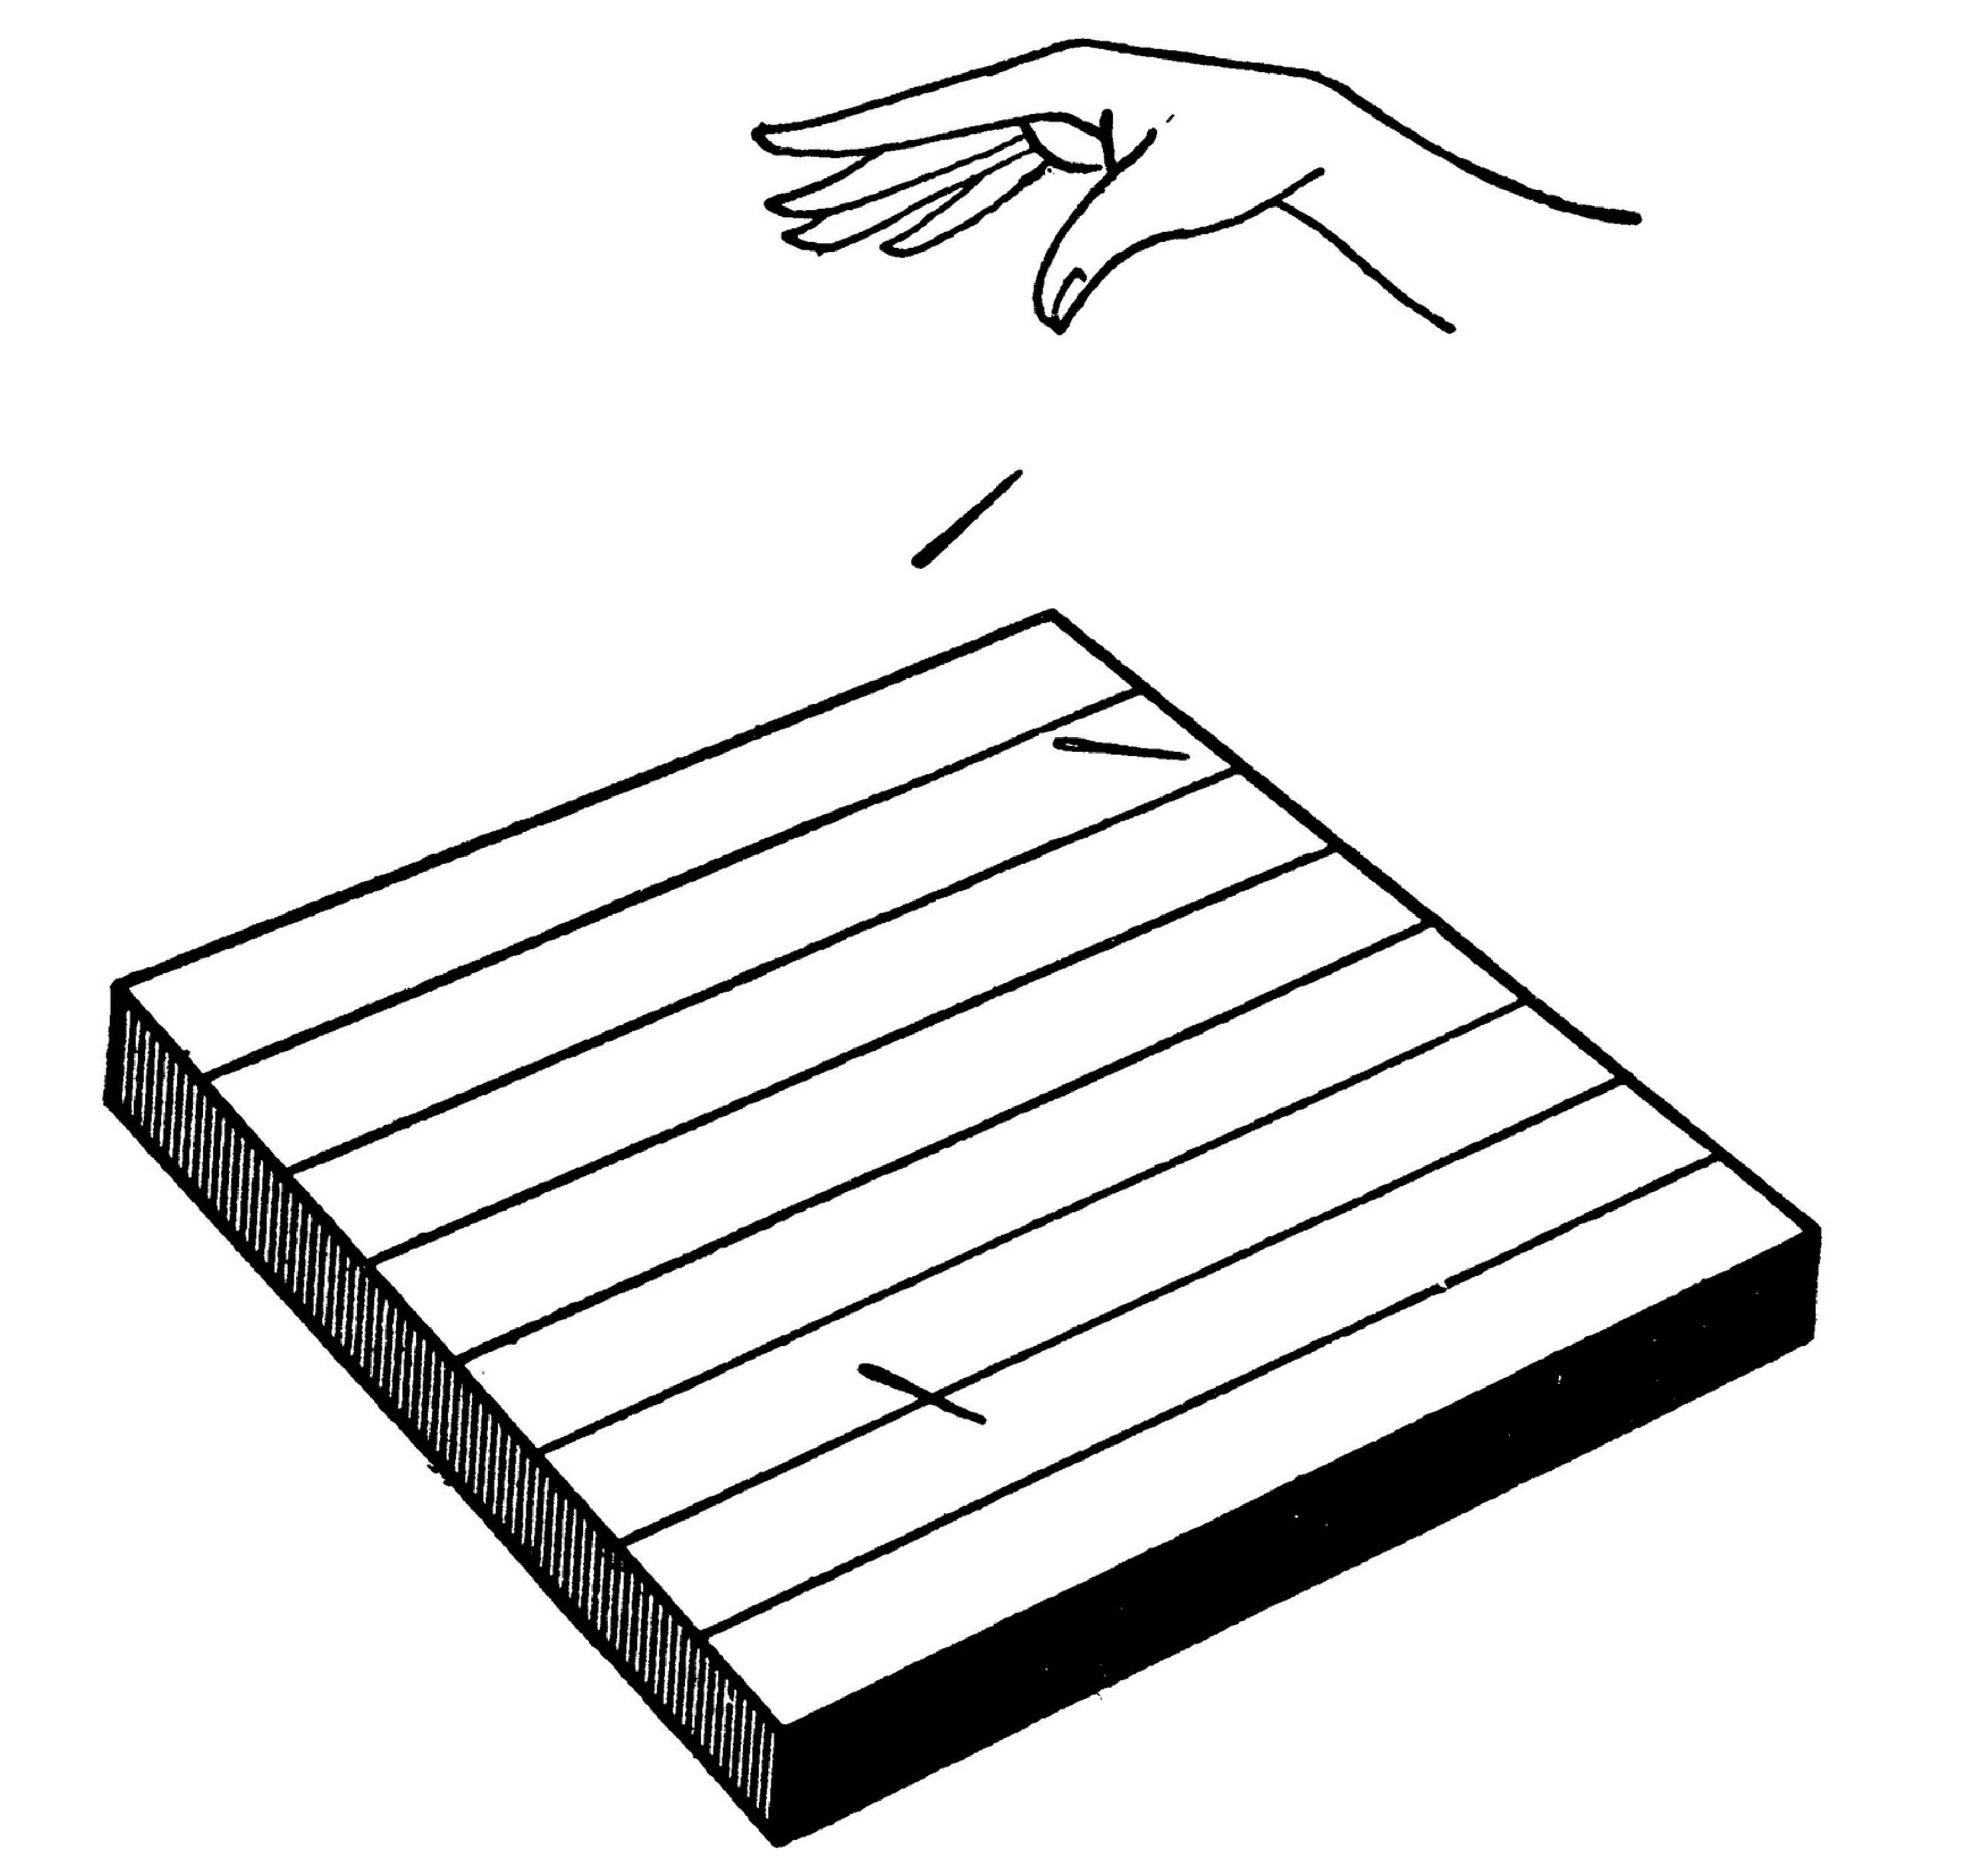
\includegraphics[scale=0.10]{aguja-de-buffon.eps}
\end{figure}
\end{frame}
\begin{frame}
\frametitle{La aguja de Buffon}
Resulta que si la distancia entre las líneas paralelas es la misma que la longitud $\ell$ de la aguja lanzada, el número de veces que la aguja cae atravesando las líneas (luego de un gran número de lanzamientos), nos servirá para calcular el valor de $\pi$.
\end{frame}
\subsection{Aproximación al valor de $\pi$}
\begin{frame}
\frametitle{Aproximación al valor de $\pi$}
De esa manera: 
\[  \pi = \dfrac {2N}{A} \]
siendo $N$ el número total de intentos y $A$ el número de veces que la aguja ha cruzado alguna línea.
\end{frame}
\begin{frame}
\frametitle{Primer problema de tarea}
Considera el caso en el que la longitud de la aguja es igual a la separación entre las rayas, es decir $\ell = h$.
\\
\bigskip
Si la aguja cruza una línea de manera oblicua, es decir, existe un ángulo de inclinación con respecto a la línea, puedes deducir la relación a partir de la \enquote{función} que describe el caso de las agujas que tocan las líneas.
\end{frame}
\begin{frame}
\frametitle{Segundo problema de tarea}
Una vez que has deducido el problema, implementa en python un programa que calcule el valor aproximado de $\pi$, a partir del número de lanzamientos, y el número de agujas que cruzan una línea.
\\
\bigskip
En las siguientes gráficas verás los resultados cuando se realiza el lanzamiento de $10^{2}, 10^{3}, 10^{4}, 10^{5}, 10^{6}$ agujas.
\end{frame}
% \begin{frame}
% \frametitle{Configuración para el problema de la aguja}
% \begin{figure}[fragile]
% \begin{tikzpicture}{font=\small}
% 	\draw [thick] (0, 0) -- (7,0);
% 	\draw [thick] (0, 4) -- (7,4);
% 	\draw [<->] (1,0) -- node[left] {Distancia entre líneas = 1}(1, 4);
% \end{tikzpicture}
% \end{figure}
% \end{frame}
\begin{frame}
\frametitle{Solución con python}
\begin{figure}
  \centering
  \includegraphics[scale=0.6]{aproximacionPi_100.eps}
\end{figure}
\end{frame}
\begin{frame}
\frametitle{Solución con python}
\begin{figure}
  \centering
  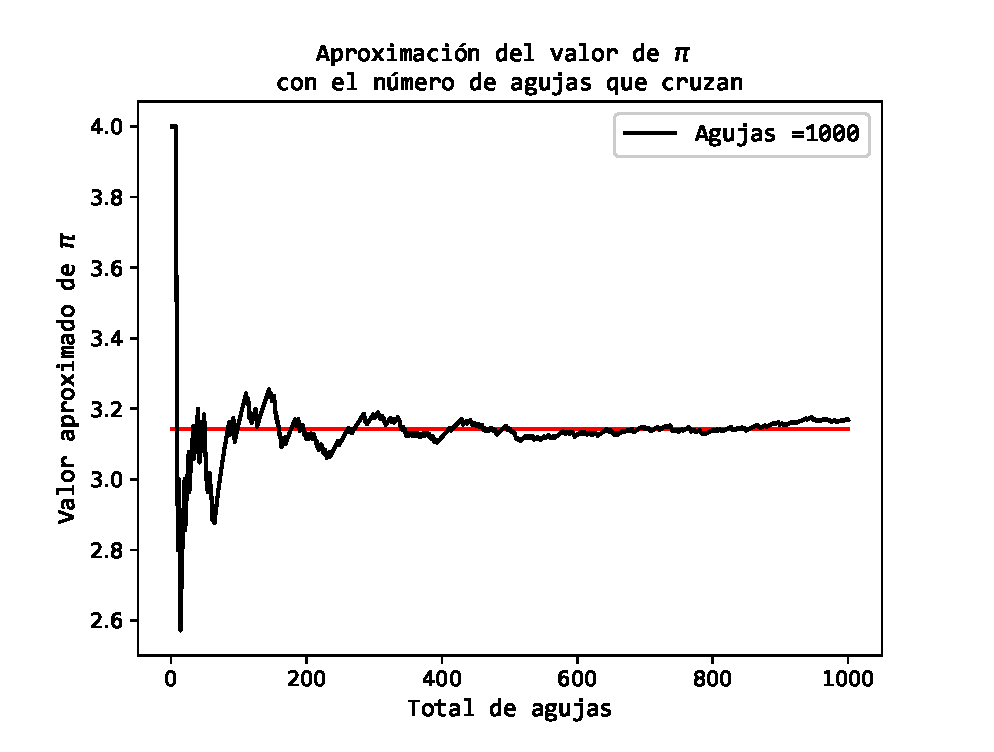
\includegraphics[scale=0.6]{aproximacionPi_1000.eps}
\end{figure}
\end{frame}
\begin{frame}
\frametitle{Solución con python}
\begin{figure}
  \centering
  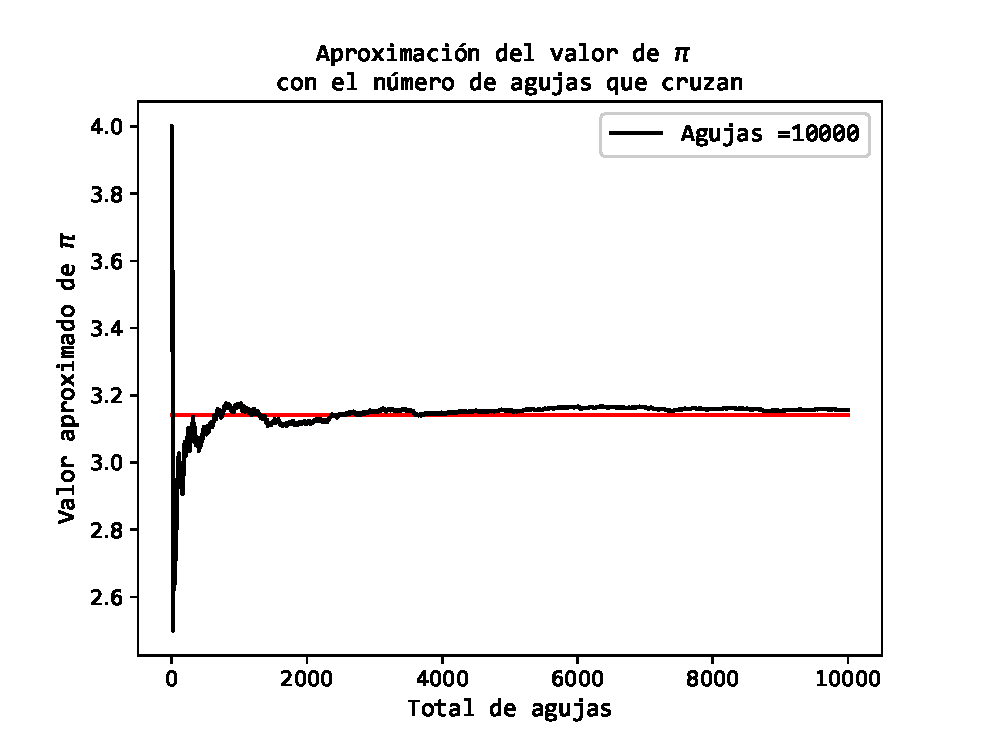
\includegraphics[scale=0.6]{aproximacionPi_10000.eps}
\end{figure}
\end{frame}
\begin{frame}
\frametitle{Solución con python}
\begin{figure}
  \centering
  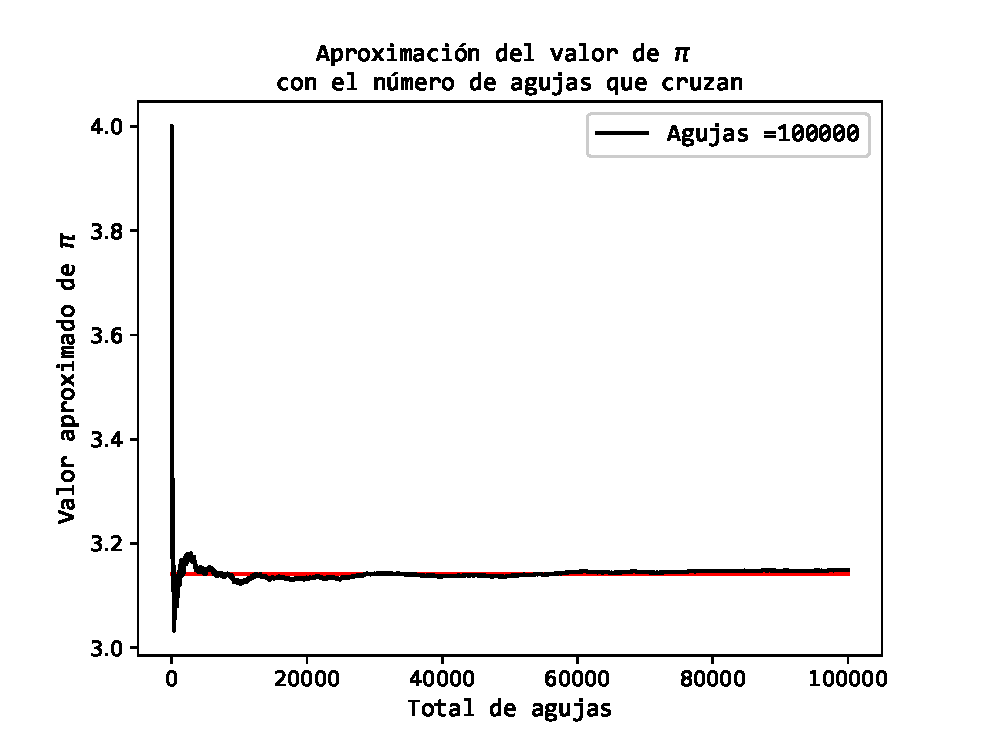
\includegraphics[scale=0.6]{aproximacionPi_100000.eps}
\end{figure}
\end{frame}
\begin{frame}
\frametitle{Solución con python}
\begin{figure}
  \centering
  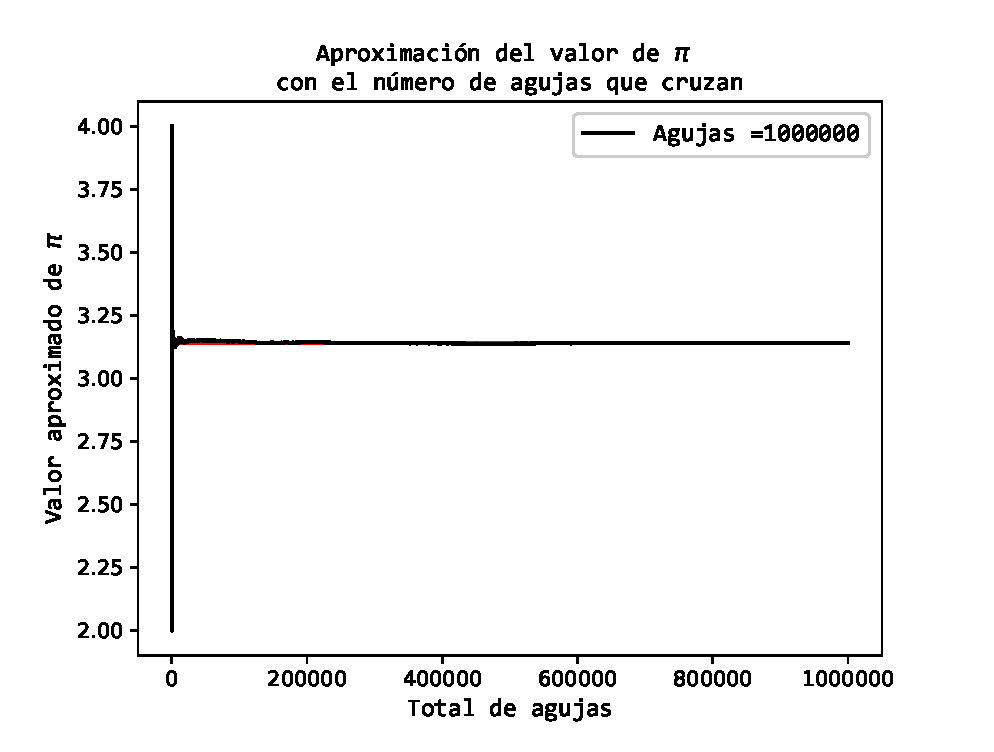
\includegraphics[scale=0.6]{aproximacionPi_1000000.eps}
\end{figure}
\end{frame}
\end{document}